% ------------ begin cheatsheet
\documentclass[a4paper]{article}
\usepackage[a4paper,margin=0.1in]{geometry}
\usepackage{multicol}

\usepackage{amsmath, amssymb}
\usepackage{enumitem}
\usepackage{graphicx}

\usepackage{ulem}
\usepackage{makecell}

% math
\newcommand{\abs}[1]{\left\lvert#1\right\rvert}

% envs
\newcommand{\ol}[1]{\begin{enumerate}#1\end{enumerate}}
\newcommand{\oll}[1]{\begin{enumerate}[leftmargin=*]#1\end{enumerate}}
\newcommand{\ul}[1]{\begin{itemize}#1\end{itemize}}
\newcommand{\ull}[1]{\begin{itemize}[leftmargin=*]#1\end{itemize}}

\graphicspath{ {./images/} }
\pagestyle{empty}
\setlength{\columnseprule}{0.2pt}

% reduce spacing before and after headers
\newcommand{\uppercaseandunderline}[1]{\uline{\uppercase{#1}}}

\makeatletter
\renewcommand{\section}{
  \@startsection{section}{1}{0pt}{1.5ex}{1.5ex} {\raggedleft\normalfont\normalsize\bfseries\uppercaseandunderline}}
\renewcommand{\subsection}{
  \@startsection{subsection}{2}{0pt}{1ex}{1.2ex} {\raggedleft\normalfont\small\bfseries\fbox}}
\renewcommand{\subsubsection}{
  \@startsection{subsubsection}{3}{0pt}{1ex}{.8ex} {\raggedleft\normalfont\footnotesize\bfseries\uline}}
\renewcommand{\paragraph}{
  \@startsection{paragraph}{4}{0pt}{1ex}{-0.8em}{\normalfont\bfseries}}

\setlist{itemsep=0.2pt, topsep=2pt}

% ------------ end cheatsheet

% ------------ begin code
\usepackage{xcolor}
\definecolor{dkgreen}{rgb}{0,0.6,0}
\definecolor{gray}{rgb}{0.5,0.5,0.5}
\definecolor{mauve}{rgb}{0.58,0,0.82}
\definecolor{lg}{rgb}{0.9,0.9,0.9}

% code environment
\usepackage{listings}
\lstset{
  %frame=tb, % adds top and bottom border
  aboveskip=1mm,
  belowskip=1mm,
  showstringspaces=false,
  columns=flexible,
  basicstyle={\footnotesize\ttfamily},
  numberstyle=\color{gray},
  keywordstyle=\color{blue}\textbf,
  commentstyle=\color{dkgreen},
  stringstyle=\color{mauve},
  breaklines=true,
  breakatwhitespace=true,
  backgroundcolor=\color{lg},
  tabsize=4
}
\newcommand{\ic}[1]{\lstinline{#1}}

% ------------ end code

\usepackage{array}
\newcolumntype{C}{>{$}c<{$}} % math-mode version of "c" column type

% Skipped:
% Lec 13 probability theory stuff

\begin{document}
\lstset{language=Java}
\footnotesize
% --- MIDTERM CONTENT ---
% First page
\begin{multicols}{3}
  \lstset{language=Java, backgroundcolor=\color{lg}}
  \section*{Java}
    \ull {
      \item Use \ic{Object.equals(Object o)} to compare
      \item String concatenation takes $O(\text{length})$
    }
  \section*{Big-O notation}
    \paragraph{Upper bound} $T(n) = O(f(n))$ if for some $c > 0$ and $n_0 > 0$,
      \[ T(n) \leq c f(n) \]
      for all $n > n_0$.
    \paragraph{Lower bound} $T(n) = \Omega(f(n))$ if for some $c > 0$ and $n_0 > 0$,
      \[ T(n) \geq c f(n) \]
      for all $n > n_0$.
    \paragraph{Tight bound} $T(n) = \Theta(f(n))$ if
      \[ T(n) = O(f(n)) \quad\text{and}\quad T(n) = \Omega(f(n)) \]
    \paragraph{Properties}
      Let $T(n) = O(f(n))$ and $S(n) = O(g(n))$.
      \oll {
        \item If $T(n)$ is a polynomial of degree $k$ then
          \[ T(n) = O(n^k) \]
        \item Addition: $T(n) + S(n) = O(f(n) + g(n))$
        \item Multiplication: $T(n) \times S(n) = O(f(n) \times g(n))$
        \item Max: $\max(T(n), S(n)) = O(f(n) + g(n))$
        \item Composition: $T(S(n)) = O(f \circ g(n))$ only if both functions are increasing
      }
    \paragraph{Overview}
      \begin{align*}
        1 < \log n < \sqrt{n} < n < n \log n \\ < n^2 < n^3 < 2^n < 2^{2n} < n! < n^n
      \end{align*}
    \paragraph{Stirling's approximation}
      $ n! \approx \sqrt{2 \pi n} \left(\dfrac{n}{e}\right)^n $ \\
      Used to show that $\log(n!) = O(n \log n)$
    \paragraph{Geometric series}
      \[ S_n = a + ar + ar^2 + \cdot + ar^{n-1} = \frac{a(1-r^n)}{1-r} \]
    \paragraph{Harmonic series}
      $ \sum_{i=1}^\infty \frac{1}{i} = O(\log n) $
    \paragraph{Logarithm change of base}
      $ \log_b a = \dfrac{\log_x b}{\log_x a} $
    \paragraph{Master theorem} Comparing $f(n)$ with $n^{\log_b(a)}$ as polynomials, for $a \geq 1$ and $b > 1$,
      \[
        \begin{aligned}
          & T(n) \\
          &= a T\left( \frac{n}{b} \right) + f(n) \\
          &= \begin{cases}
               \Theta(n^{\log_b(a)}) & \text{if } f(n) < n^{\log_b(a)} \\
               \Theta(n^{\log_b(a)} \log n) & \text{if } f(n) = n^{\log_b(a)} \\
               \Theta(f(n)) & \text{if } f(n) > n^{\log_b(a)} \\
             \end{cases}
        \end{aligned}
      \]
  \section*{Algorithms} \noindent
    (with binary search as example algo)
    \paragraph{Precondition} Fact before algorithm runs.
      e.g. Array is sorted
    \paragraph{Postcondition} Fact when algorithm ends.
      e.g. If element in array, then \ic{A[begin] = key}
    \paragraph{Invariant} Relationship between variables that is always true
    \paragraph{Loop invariant} Invariant at beginning/end of loop
      e.g. \ic{A[begin] <= key <= A[end]}, i.e. key is in range
    \subsection*{Peak finding} \noindent
      Assume \ic{A[-1]} and \ic{A[n]} are \ic{-INT_MAX}.
      \begin{lstlisting}
FindPeak(A, n)
  mid = n/2
  if A[mid+1] > A[mid] then recurse on right half
  elif A[mid-1] > A[mid] then recurse on left half
  else A[mid] is a peak
      \end{lstlisting}
      If we recurse into right half, then:
      \ull {
        \item Given that \ic{A[mid] < A[mid+1]} (condition for recursing into right half)
        \item Assuming no peak, then \ic{A[mid] < A[mid+1] < A[mid+2] < ... < A[n-1] > A[n] = -INT_MAX}, i.e. \ic{A[n-1]} is a peak
        \item Hence peak must exist
      }
    \subsection*{Sorting}
      \paragraph{Bubble} compare adjacent and swap to make right $>$ left
      \paragraph{Selection} find smallest element and swap it to end of sorted region
      \paragraph{Insertion} swap each new element until it is correctly placed within sorted region
      \paragraph{Small arrays} Insertion sort is stable, works fast for nearly sorted arrays, has little overhead.
      \paragraph{Merge} (recursive) sort each half and merge
      \paragraph{Quicksort} (recursive) partition about a pivot
      \paragraph{In-place partitioning} $O(n)$
        \oll {
          \item Choose a random pivot (for good quicksort performance), and swap it to the start
          \item Increase \ic{lptr} while element at left $<$ pivot
          \item Decrease \ic{rptr} while element at right $>$ pivot
          \item If not yet at centre, swap pointers and repeat
        }
      \paragraph{Quicksort variations}
        \ull {
          \item Is stable only if the partitioning is stable. Requires $O(n)$ extra space to store initial indices
          \item If pivot splits by a fraction, good enough
          \item 3-way partitioning: pack duplicates in middle to eliminate duplicate elements worst case
          \item Paranoid: force a good pivot
          \item $k$-pivots: $O(k \log k)$ to sort pivots + $O(n \log k)$ to binary search the pivots to choose correct bucket to place the new item. $T(n) = O(n \log_k n \log k) = O(n \log n)$, i.e. no performance improvements
          \item 2-pivot quicksort is in practice better than 1-pivot quicksort, because of cache performance
        }
      \paragraph{Quickselect} Like quicksort, but only recurse on relevant half of partitioned array
    \subsection*{Probability}
      \paragraph{Linearity of expectation} For random variables $X$ and $Y$: $E(aX + bY) = a E(X) + b E(Y)$
      \paragraph{Expected trials} If an event $X$ has probability of success $p$, then an expected $\tfrac{1}{p}$ trials is required for 1 success.
  \section*{Trees}
    \subsection*{Binary trees}
      \ull {
        \item A binary tree is either empty, or a node pointing to two binary trees.
        \item In a \underline{balanced tree}, $h = O(\log n)$
        \item Height is no. of edges on longest path to leaf
      }
      The following operations are all $O(\log n)$:
      \paragraph{searchMin} keep going left
      \paragraph{searchMax} keep going right
      \paragraph{search, insert} go left/right depending on comparison of new key with cur key
      \paragraph{successor}
        \ull {
          \item If node has right child: \ic{right.searchMin()}
          \item Else traverse upwards until ancestor contains node in left subtree, then return ancestor
        }
      \paragraph{predecessor}
        \ull {
          \item If node has left child: \ic{left.searchMax()}
          \item Else traverse upwards until ancestor contains node in right subtree, then return ancestor
        }
      \paragraph{delete}
        \ull {
          \item 0 children: remove node
          \item 1 child: remove node, connect parent to child
          \item 2 children: delete successor (at most 1 child), replace node value with successor value
        }
      The following operations are all $O(n)$:
      \paragraph{in-order} left, self, right
      \paragraph{pre-order} self, left, right
      \paragraph{post-order} left, right, self
      \paragraph{level-order} decreasing height (BFS)
      \paragraph{Ancestor} Node $x$ is an ancestor of node $y \Leftrightarrow x$ comes before $y$ in pre-order, AND $y$ comes before $x$ in post-order.
  \subsection*{AVL trees}
    \ull {
      \item A node $v$ is \underline{height balanced} if \\
        \ic{|v.L.height - v.R.height| <= 1}
      \item Consider a height balanced tree with height $h$ and $n$ nodes.
        \ull {
          \item \textbf{At most} $h < 2 \log n$ (actually, approximately $\dfrac{1}{\log \phi} \log n$)
          \item \textbf{At least} $n > 2^{h/2}$ nodes
        }
      \item Can build AVL tree in $O(N)$ given sorted array (keep selecting median as root of subtree)
    }
    \paragraph{Balancing}
      Assume A is \underline{left-heavy}. Otherwise, if A is right-heavy, substitute ALL left, right with right, left
      \\\\
      Define B as left child of A.
      \\\\
      Case 1: B is \textbf{balanced:} \ic{rightRotate(A)}
      \begin{center}
        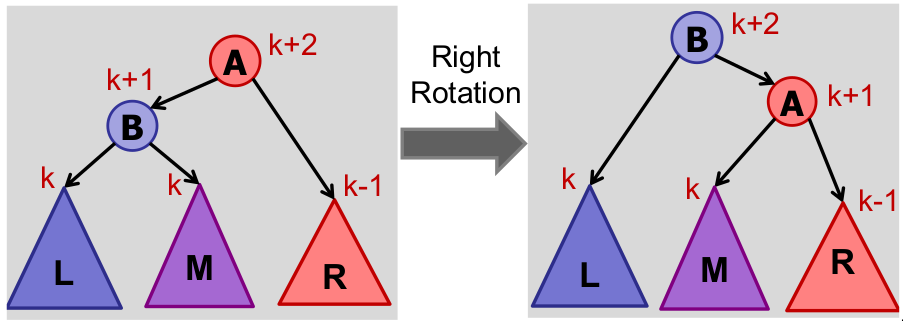
\includegraphics[width=0.29\textwidth]{AVL_Case_1}
      \end{center}
      Case 2: B is \textbf{left-heavy:} \ic{rightRotate(A)}
      \begin{center}
        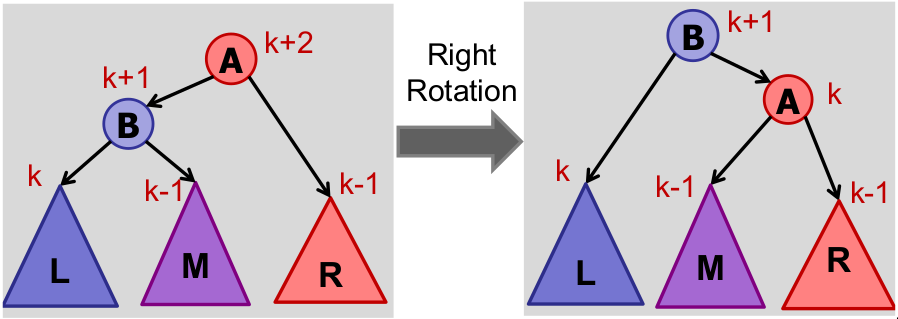
\includegraphics[width=0.29\textwidth]{AVL_Case_2}
      \end{center}
\end{multicols}

\vspace{-1.3\baselineskip}
\hrulefill
\vspace{-1.0\baselineskip}

% Recurrence time complexity
\begin{multicols}{3}
  % hacky solution to reduce unnecessary vertical spacing
  {\centering
    $O(1)$ work \\ \vspace{.2cm}
    $ \displaystyle
    \begin{aligned}
      T(n) &= T (\tfrac{n}{k}) + O(1) = O(\log n) \\
      T(n) &= kT (\tfrac{n}{k}) + O(1) = O(n) \\
      T(n) &= kT (\tfrac{n}{2k}) + O(1) = O(\sqrt n)
    \end{aligned}
    $
  \par}
  {\centering
    Not $O(1)$ work \\ \vspace{.2cm}
    $ \displaystyle
    \begin{aligned}
      T(n) &= T (\tfrac{n}{k}) + O(n) = O(n) \\
      T(n) &= kT (\tfrac{n}{k}) + O(n) = O(n \log n) \\
      T(n) &= kT (\tfrac{n}{k}) + O(n \log n) = O(n \log^2 n)
    \end{aligned}
    $
  \par}
  {\centering
    Subtract in recurrence \\ \vspace{.2cm}
    $ \displaystyle
      \begin{aligned}
        T(n) &= T(n-c) + O(n) = O(n^2) \\
        T(n) &= 2T(n-1) + O(1) = O(2^n) \\
        T(n) &= T(n-1) + T(n-2) + O(1) = O(\phi^n)
      \end{aligned}
    $
  \par}
\end{multicols}

% Sort summary
\begin{center}
  \begin{tabular}{ |c|C|C|C|c|C|c| }
    \hline
    \textbf{Sort} & \textbf{Best} & \textbf{Average} & \textbf{Worst} & \textbf{Stable} & \textbf{Memory} & \textbf{Invariant (after $k$ iterations)} \\ \hline
    Bubble & \Omega(n) & O(n^2) & O(n^2) & \checkmark & O(1) & last $k$ elements in correct final position \\ \hline
    Selection & \Omega(n^2) & O(n^2) & O(n^2) & $\times$ & O(1) & first $k$ elements in correct final position \\ \hline
    Insertion & \Omega(n) & O(n^2) & O(n^2) & \checkmark & O(1) & (original) first $k$ elements in relative sorted order \\ \hline
    Merge & \Omega(n \log n) & O(n \log n) & O(n \log n) & \checkmark & O(n) & subarray is sorted \\ \hline
    Quick & \Omega(n \log n) & O(n \log n) & O(n^2) & $\times$ & O(1) & pivot is in correct final position \\ \hline
  \end{tabular}
\end{center}

\pagebreak

% Second page onwards
\begin{multicols}{3}
      \noindent
      Case 3: B is \textbf{right-heavy:} \\
        \ic{leftRotate(A.left); rightRotate(A)}
      \begin{center}
        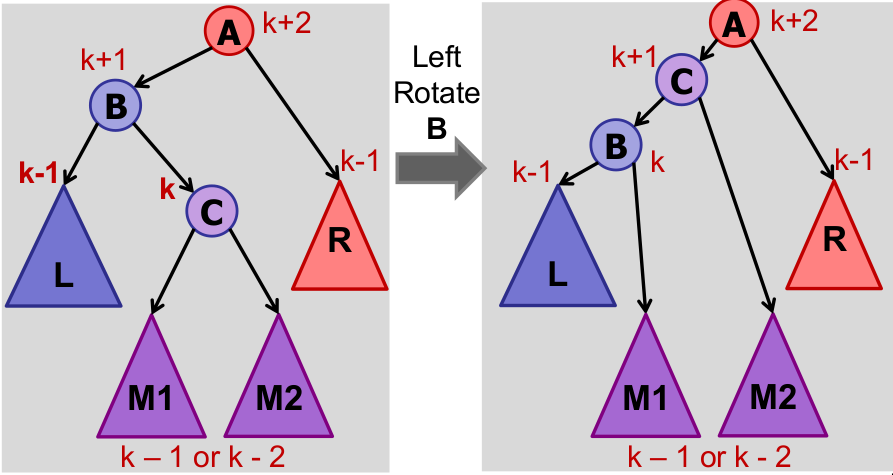
\includegraphics[width=0.29\textwidth]{AVL_Case_3a}
        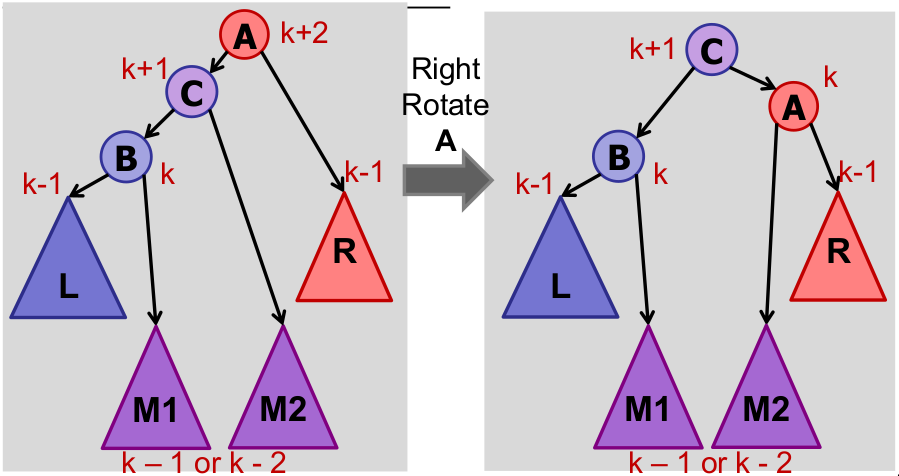
\includegraphics[width=0.29\textwidth]{AVL_Case_3b}
      \end{center}
      Update weights after \ic{rightRotate(A)}
      \begin{center}
        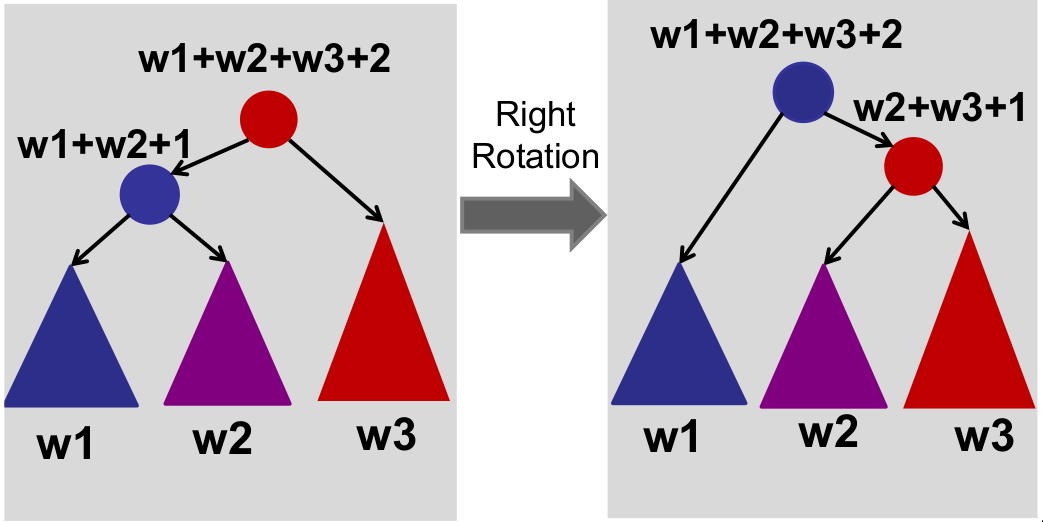
\includegraphics[width=0.29\textwidth]{AVL_weights}
      \end{center}
      Update max after \ic{rightRotate(A)}
      \begin{center}
        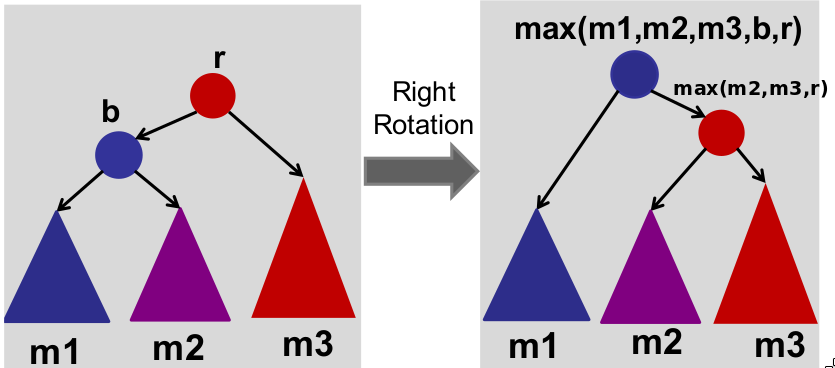
\includegraphics[width=0.29\textwidth]{AVL_max}
      \end{center}
      \ull {
        \item Insertion: max 2 rotations
        \item Deletion: max $O(\log n)$ rotations
      }
    \paragraph{Rank of node} Position in in-order
      \begin{lstlisting}
rank(node):
  rank = node.L.weight + 1
  while node != null
    if node is right child
      rank += node.parent.L.weight + 1
    node = node.parent
  return rank
      \end{lstlisting}
  \subsection*{Trie} \noindent
    search, insert: $O(L)$, space: $O\Big(\sum L + \text{overhead}\Big)$
  \subsection*{Order Statistics}
    \paragraph{Find $k$th smallest element} Quicksort but only recurse on relevant side - $O(n)$
    \paragraph{Dynamic} Augment with size of subtree at each node, use rank algo
  \subsection*{Interval Tree} \noindent
    Each node stores an interval (left endpoint as key), augmented with max right endpoint in subtree
    \paragraph{Search} $O(\log n)$
      \oll {
        \item If value in node interval, return node
        \item If \ic{value > node.left.max}, recurse right
        \item Else recurse left
      }
      \paragraph{All-overlaps} If we want to find all $k$ intervals that contain value - $O(k \log n)$
      \oll {
        \item Search for interval
        \item Add to list and delete interval
      }
  \subsection*{Orthogonal Range Searching}
    \ull {
      \item Leaf nodes contain points
      \item Internal nodes contain max in left subtree
      \item Build tree: $O(n \log n)$, Space: $O(n)$
    }
    \paragraph{Search} Find number of points in range $[a, b]$ - $O(k + \log n)$, where $k$ is number of points found
      \oll {
        \item Find split node, highest node with key in range $[a, b]$
        \item Do left child traversal
          \ull {
            \item If node in query range, then add entire right subtree to list, and recurse left
            \item Else recurse right
          }
        \item Do right child traversal (similar)
      }
    \paragraph{n dimensional search}
      \ull {
        \item Recursively store $d-1$ dim range tree in each node of a 1D range tree
        \item Build tree: $O(n \log^{d-1} n)$, Query: $O(\log^d n + k)$
        \item Space: $O(n \log^{d-1} n)$, 2D tree Rotate: $O(n)$
      }
  \subsection*{$k$-d tree}
    \ull {
      \item Stores coordinates in $x-y$ plane
      \item Levels alt. between splitting plane by $x$ or $y$
    }
    \paragraph{Search node} $O(\log n)$
      \oll {
        \item If horizontal split, compare $x$-coordinate
        \item If vertical split, compare $y$-coordinate
        \item $O(h)$ time
      }
    \paragraph{Search min} $O(\sqrt n)$ (e.g. min $x$)
      \oll {
        \item If horizontal split, recurse left child
        \item If vertical split, recurse on both children
        \item $T(n) = 2T(n/4) + O(1)$
      }
    \paragraph{Build} $O(n \log n)$
      \oll {
        \item Choose either $x$ or $y$.
        \item Quickselect median of $x$ or $y$: $O(n)$
        \item Split array into two halves using median \\
          Partioning: $O(n)$
      }
  \subsection*{$(a,b)$-tree}
    \begin{center}
      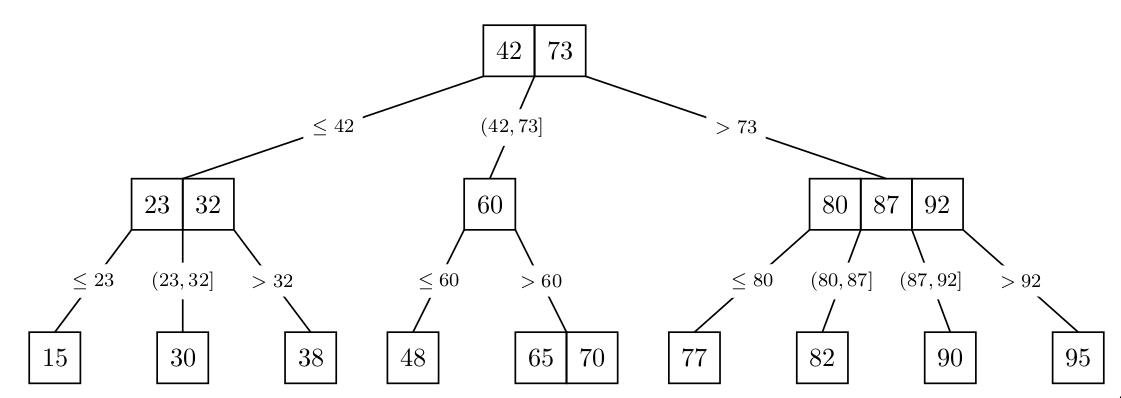
\includegraphics[width=0.32\textwidth]{AB_tree}
      \\
      Sample $(2,4)$-tree
    \end{center}
    \paragraph{Rules}
      \oll {
        \item $(a,b)$ child policy
          \begin{center}
            \begin{tabular}{ |c|c|c|c|c| }
              \hline
              & \multicolumn{2}{c|}{\# Keys} & \multicolumn{2}{c|}{\# Children} \\ \hline
              Node & Min & Max & Min & Max \\ \hline
              Root & 1 & $b-1$ & 2 & $b$ \\ \hline
              Internal & $a-1$ & $b-1$ & $a$ & $b$ \\ \hline
              Leaf & $a-1$ & $b-1$ & 0 & 0 \\ \hline
            \end{tabular}
          \end{center}
        \item A non-leaf node must have one more child than its number of keys
        \item All leaf nodes must all be at the same depth
      }
    \paragraph{Definitions}
      \ull {
        \item Key range: Range of keys allowed in a subtree (wrt parent)
        \item Key list: List of keys in node (assume sorted)
        \item Tree list: List of children
      }
    \paragraph{$B$-tree} simply $(B,2B)$ trees
    \paragraph{Search} $O(\log n)$:
      \ull {
        \item $O(\log b)$ binary search keylist for subtree containing the key to search
        \item Repeat along height of $O(\log_a n)$
      }
    \paragraph{Insert} $O(\log n)$: Like search, then perform split/merge as necessary
      \ull {
        \item Proactive: preemptively split nodes at full capacity (only applies if $b \geq 2a$)
        \item Passive: insert then check (potentially splitting all the way to root)
      }
    \paragraph{Delete} $O(\log n)$: Like search, then perform split/merge as necessary
    \paragraph{Split}
      \begin{center}
        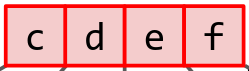
\includegraphics[width=0.14\textwidth]{B-tree/split_before}
        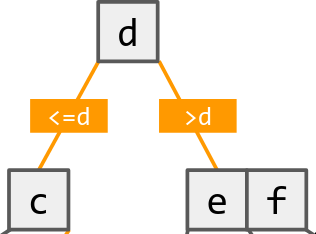
\includegraphics[width=0.14\textwidth]{B-tree/split_after}
      \end{center}
      \oll {
        \item Pick median key of overfull range $z$ as new split key $k$
        \item Put $k$ into parent
        \item Split $z$ into LHS and RHS of $k$
        \item If parent is overfull, \ic{split(parent)}
      }
    \paragraph{Merge}
      \begin{center}
        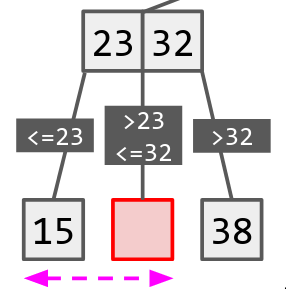
\includegraphics[width=0.14\textwidth]{B-tree/merge_before}
        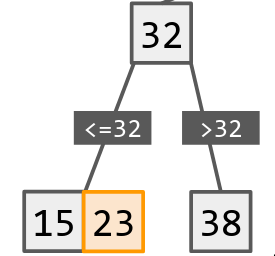
\includegraphics[width=0.14\textwidth]{B-tree/merge_after}
      \end{center}
      Let $d$ be deleted node, and $l$ be left sibling of $d$. Assume keylist of $l$ and $d$ have $< b-1$ keys in total. Otherwise use share below
      \oll {
        \item Pick key $k$ from parent, on left of $d$
        \item Move $k$ to keylist of $l$
        \item Merge $d$ keylist, treelist into $l$
        \item Delete $d$
      }
    \paragraph{Share} \ic{merge(l, d)}; then split newly combined node
\section*{Hashing}
  \paragraph{Hash functions}
    \ull {
      \item Maps universe to keys in $\{1,\cdots,m\}$
      \item Store item with key $k$ in bucket $hash(k)$
      \item Since universe size larger, collisions inevitable by pigeonhole principle
    }
  \paragraph{Simple uniform hashing assumption}
    \oll {
      \item Each key has equal probability of being mapped to each bucket
      \item Each key is mapped independently to each bucket
    }
  \paragraph{Uniform hashing assumption}
    \ull {
      \item Stronger version of SUHA property 2: Every key is mapped independently to every permutation.
    }
  \subsection*{Java implementation}
    \paragraph{\ic{java.util.Map} interface}
      \ull {
        \item Does not allow duplicate or mutable keys
      }
    \paragraph{hashCode}
      \ull {
        \item Always returns the same value, if the object hasn't changed
        \item If two objects are equal, then they return the same hashCode
        \item Must redefine \ic{.equals()} to be consistent with hashCode
      }
    \paragraph{equals}
      \ull {
        \item Reflexive: $x = x$
        \item Symmetric: $x = y \Rightarrow y = x$
        \item Transitive: $(x = y) \land (y = z) \Rightarrow x = z$
        \item Consistent: always returns same answer
        \item Null: \ic{x.equals(null) == false}
      }
  \subsection*{Chaining} \noindent
    Assume $n$ keys have been inserted into hash table of size $m$.
    \ull {
      \item Each bucket $c$ stores linked list of items with $hash(k) = c$
      \item Total space: $O(n + m)$
    }
    \paragraph{Insert}
      \ull {
        \item Allow duplicate keys: $O(1 + hash) = O(1)$
        \item Don't allow dupe keys $\Rightarrow$ search on insert
      }
    \paragraph{Search}
      \ull {
        \item Without SUHA (assume all items have same hash): $O(n + hash) = O(n)$
        \item With SUHA (consider expected case): $O(1 + hash + n/m)$
        \item Choose good $m$, e.g. $m=2n$: $O(1 + hash)$
      }
    \paragraph{Expected max cost of $n$ inserts}
      \ull {
        \item $O(\log n) = \Theta( \frac{\log n}{\log \log n} )$
      }
  \subsection*{Open addressing}
    \subsubsection*{Properties}
      \ull {
        \item NULL = empty, DELETED = deleted
        \item Insert: probe a sequence of buckets until NULL/DELETED
        \item Search: probe same sequence until found/NULL
        \item Delete: find key to delete, set bucket to DELETED
      }
    \subsubsection*{Linear probing} \noindent
      Define new hash function $h$ such that
      \[ h(key, i) = k(key, 1) + i \pmod m \]
      where $i$ is the number of collisions.
      \ull {
        \item SUHA property 1: $h(key, i)$ is a permutation of $\{1, \cdots, m\}$
        \item Does NOT satisfy stronger version of SUHA property 2, because linear probing requires a circular permutation of $\{1, \cdots, m\}$
      }
      \paragraph{Performance}
        \ull {
          \item Clustering: If table is 1/4 full, $\exists$ clusters of size $\Theta(\log n)$, which ruins constant-time performance
          \item In practice, caching makes this much faster
          \item Expected cost of an operation, $E[\text{\# probes}] \leq \dfrac{1}{1-\alpha}$
          \item $\alpha$ is average no. of items per bucket, $n/m$.
        }
  \subsection*{Double hashing} \noindent
    Given two hash functions $f, g$, define:
    \[ h(k, i) = f(k) + i \cdot g(k) \pmod m \]
    \ull {
      \item If $g(k)$ is relatively prime to $m$, then $h(k,i)$ hits all buckets.
      \item If $m = 2^r$, then choose $g(k)$ odd.
    }
  \subsection*{Table size} \noindent
    Let $n$ be the number of elements in the hash table. Let $m$ be the size of the hash table.
    \paragraph{Growing table} Time: $O(m_\text{old} + m_\text{new} + n)$
      \begin{center}
        \begin{tabular}{ |c|c|c| }
          \hline
          \textbf{growth} & \textbf{resize} & \textbf{insert $n$ items} \\ \hline
          increment & $O(n)$ & $O(n^2)$ \\ \hline
          double & $O(n)$ & $O(n)$ \\ \hline
          square & $O(n^2)$ & $O(n^2)$ \\ \hline
        \end{tabular}
      \end{center}
    \paragraph{Shrinking table}
      \ull {
        \item If we choose to shrink when table at half capacity, we have a scenario. Consider $n=200, m=100$. Delete causes a shrink, insert causes a grow, repeat.
        \item Hence, we choose the following:
          \ull { 
            \item If $(n == m)$, then $m = 2m$
            \item If $(n < m/4)$, then $m = m/2$
            \item Growth $\Rightarrow \geq m/2$ new items are added $\Rightarrow$ can pay for growing
            \item Shrink $\Rightarrow \geq m/4$ items are deleted $\Rightarrow$ can pay for shrinking
          }
      }

% --- FINALS CONTENT ---
\section*{Amortized analysis} \noindent
  An op has amortized cost $T(n)$ if for every integer $k$, the cost of $k$ ops is $\leq k T(n)$.
  \paragraph{Hash table resizing} Inserting $k$ elements into a hash table with resizing takes $O(k)$, so insert has amortized $O(1)$ cost.
  \paragraph{Binary counter} Increment has amortized $O(1)$ cost
\section*{Graphs}
  \paragraph{Graph}
    \ull {
      \item Nonempty set of objects (nodes) with a set of relations (edges) 
      \item Each edge connects two nodes
    }
  \paragraph{Multigraph} Two nodes may be connected by more than one edge
  \paragraph{Hypergraph} Each edge connects $\geq 2$ nodes
  \paragraph{(Simple) path}
    \ull {
      \item Set of edges connecting two nodes
      \item Path intersects each node at most once
    }
  \paragraph{Cycle} ``Path'' where first node = last node
  \paragraph{Degree of node} Number of adjacent edges
  \paragraph{Degree of graph} Max degree over all nodes
  \paragraph{Diameter of graph} Max distance between two nodes in a graph, using shortest path
  \subsection*{Types of graphs}
    \paragraph{Connected graph} Every pair of nodes is connected by a path
    \paragraph{Disconnected graph} Some pair of nodes is not connected by a path
    \paragraph{Tree} Connected graph with no cycles
    \paragraph{Forest} Graph with no cycles
    \paragraph{Star} One central node, all edges connect center to other nodes
    \paragraph{Clique (complete graph)} All pairs of nodes are connected with an edge
    \paragraph{Line} Tree with degree 2
    \paragraph{Cycle} Entire graph is a cycle
    \paragraph{Bipartite}
      \ull {
        \item Nodes can be divided into two sets, with no edges between nodes of the same set
        \item Does not have odd-length cycles
      }
    \vspace{-3mm}
    \begin{center}
      \begin{tabular}{ |c|c|c| }
        \hline
        \textbf{Type} & \textbf{Degree} & \textbf{Diameter} \\ \hline
        Star & $n-1$ & 2 \\ \hline
        Clique & $n-1$ & 1 \\ \hline
        Line & 2 & $n-1$ \\ \hline
        Cycle & 2 & $n/2$ or $n/2 - 1$ \\ \hline
      \end{tabular}
    \end{center}
    \vspace{-2mm}
  \subsubsection*{Planar graphs} \noindent
    Can be drawn on 2D plane without edges crossing
    \paragraph{Face} Area bounded by edges (outer, infinite area is also a face)
    \paragraph{Euler's formula} $V-E+F=2$
  \subsubsection*{DAGs}
    \paragraph{Directed graph} Graph with directed edges
    \paragraph{In-degree} Number of incoming edges
    \paragraph{Out-degree} Number of outgoing edges
    \paragraph{DAG} Directed graph with no cycles
  \subsection*{Representation}
    \paragraph{Adjacency list} Space: $O(V+E)$
      \ull {
        \item Nodes: stored in array, edges: linked list per node
        \item Only stores outgoing edges for directed graphs
      }
    \paragraph{Adjacency matrix} Space: $O(V^2)$
      \ull {
        \item 2D array, where $A[v][w] = e(v,w)$
        \item $A^k$ represents all length $k$ paths
        \item Symmetric $\iff$ undirected graph
      }
  \subsection*{Searching (Unweighted)}
    \paragraph{BFS} $O(V + E)$, using adjacency list
      \ull {
        \item Uses a queue
        \item Each node is visited once, and each neighbour is only enumerated once.
        \item BFS parent edges form a shortest path tree (from root)
      }
    \paragraph{DFS} $O(V + E)$, using adjacency list
      \ull {
        \item Uses a stack
        \item DFS called once per node, and each neighbour is only enumerated once.
        \item DFS parent edges form a tree
      }
  \subsection*{Topological ordering} \noindent
    Given a DAG, find a total ordering of nodes, where all edges point forwards.
    \paragraph{Idea 1} DFS with post-order processing: $O(V + E)$
      \ull {
        \item Perform usual DFS
        \item Add a node to the topo-order (in reverse order) during the post-order.
      }
    \paragraph{Idea 2} Kahn's algorithm: $O(V + E)$
      \ull {
        \item Let $S = $ all nodes in $G$ that have no incoming edges. $S$ is nonempty because $G$ is a DAG.
        \item Dequeue $v$ from $S$
          \ull {
            \item Add $v$ to topo-order
            \item Remove edges adjacent to $v$
            \item If any neighbours have no incoming edges, add to $S$
          }
        \item Repeat until $G$ is empty
      }
      We can apply the same idea considering in-degree instead.
  \subsection*{Connected components}
    \paragraph{Undirected graph}
      \ull {
        \item Vertex $v$ and $w$ are in the same connected component $\iff$ there is a path from $v$ to $w$
        \item There is a set $\{v_1, v_2, \cdots, v_k\}$ where there is no path from $v_i$ to $v_j \iff$ there are $k$ connected components
      }
    \paragraph{Strongly connected components} (Only applies to directed graphs) A component is strongly connected if for every vertex $v$ and $w$, there is a path from $v$ to $w$, and from $w$ to $v$.
    \paragraph{Graph of strongly connected components} If we replace each strongly connected component with a supernode, then the graph of the supernodes is acyclic.
  \subsection*{Shortest paths}
    \paragraph{$\Delta$ inequality} $\delta(S,C) \leq \delta(S,A) + \delta(A,C)$
    \subsubsection*{Bellman-Ford}
      \paragraph{Algorithm} $O(VE)$
        \ull {
          \item Maintain distance estimate for every node
          \item Repeat $\abs{V}-1$ times: relax every edge
          \item If one iteration does not relax any edge, we can terminate early
        }
      \paragraph{Relax}
        \begin{lstlisting}
void relax(int u, int v) {
  if (dist[v] > dist[u] + weight(u,v))
    dist[v] = dist[u] + weight(u,v);
}
        \end{lstlisting}
      \paragraph{Properties}
        \ull {
          \item $k$-hop estimate for node $v$ is correct after $k$ iterations, only if $v$ is on the shortest path tree rooted at source $s$
          \item After $k$ iterations, gives all shortest paths within $k$ hops from start
          \item Works with negative edges
          \item Does not work with negative cycle, but if run for $\abs{V}$ iterations, and estimate changes in the last iteration, then negative weight cycle exists
          \item Given a set of distance estimates, we can run 1 iteration of Bellman-Ford ($O(E)$), and if the distance estimates do not change, then the distance estimates are accurate
          \item If edge weights are all same, then use BFS and multiply the answer by the edge weight
        }
    \subsubsection*{Dijkstra}
      \paragraph{Algo} $O((E+V) \log V)$ with AVL-based PQ
        \ull {
          \item Maintain distance estimate for every node
          \item Begin with empty shortest path tree
          \item Repeat until destination reached:
            \ull {
              \item Let $v$ be the node with the minimum distance estimate so far
              \item Add $v$ to shortest path tree, mark $v$ as visited
              \item Relax all outgoing edges from $v$
            }
        }
      \paragraph{Time complexity}
        \ull {
          \item \ic{insert}: $\abs{V}$ times of $O(\log V)$
          \item \ic{deleteMin}: $\abs{V}$ times of $O(\log V)$
          \item \ic{decreaseKey}: $\abs{E}$ times of $O(\log V)$
          \item Total is $O((V+E) \log V) = O(E \log V)$
        }
      \paragraph{Properties}
        \ull {
          \item Does not work with negative edges
          \item cf. BFS/DFS, here we use a PQ
        }
    \subsubsection*{DAGs}
      \paragraph{Algorithm} $O(V+E)$
        \ull {
          \item Generate topological order - $O(V+E)$
          \item Relax edges in topological order - $O(E)$
        }
      \paragraph{Longest path} Negate edges. Shortest path in negated graph is the longest path in original graph
  \subsection*{MSTs}
    \paragraph{Spanning tree} is an acyclic subset of the edges that connects all nodes
    \paragraph{Minimum spanning tree} is a spanning tree with minimum total edge weight
    \paragraph{Cut} of a graph is a partition of the vertices into two disjoint subsets 
      \ull {
        \item An edge crosses a cut if it has one vertex in each of the two sets
      }
    \subsubsection*{Properties}
      \oll {
        \item No cycles
        \item Cut an MST, the two pieces are both MSTs.
        \item In each cycle, the max weight edge is not in the MST. Min weight edge is inconclusive.
        \item In each cut, min weight edge across cut in MST.
      }
    \subsubsection*{Generic algorithm}
      \ull {
        \item Red rule: If C is a cycle with no red arcs, then color the max weight edge in C red.
        \item Blue rule: If D is a cut with no blue arcs, then color the min weight edge in D blue.
        \item Apply red rule or blue rule to all edges. The blue edges are the edges of a MST.
      }
    \paragraph{\uline{Prim's algorithm}} $O(E \log V)$
      \ull {
        \item Maintain a cut, and store its cut-edges in a PQ.
        \item Remove min cut-edge, growing the cut by this edge (and node)
        \item Each vertex added/removed once from PQ - $O(V \log V)$
        \item Each edge has one decreaseKey - $O(E \log V)$
      }
      \paragraph{Small edge weights} $O(V+E)$ - Use array of size $k$ as PQ
    \paragraph{\uline{Kruskal's algorithm}} $O(E \log V)$
      \ull {
        \item Sort edges, and keep adding edge to set only if it does not cause a cycle
        \item Sorting - $O(E \log E) = O(E \log V)$
        \item Find/Union - $O(\log V)$ per edge
      }
      \paragraph{Small edge weights} $O(\alpha E)$ - Use array of size $k$ to sort
    \subsubsection*{All edges have same weight}
      \ull {
        \item DFS or BFS, any spanning tree is a MST
        \item MST has $V-1$ edges, cost is $k(V-1)$, where $k$ is the edge cost
      }
    \paragraph{\uline{Directed MST}} $O(E)$
      \ull {
        \item If we have a DAG with one root, for every node except the root, add min weight incoming edge
      }
    \subsubsection*{Maximum spanning tree}
      \ull {
        \item Negate edge weights and run MST, or
        \item Kruskal but sort descending
      }
\section*{Union-Find}
  \paragraph{\uline{Quick find}} \ic{int[] componentId}, flat trees
    \ull {
      \item Object ID is the array index (hash table + open addressing)
      \item Component ID is the array value
      \item $O(1)$ Find: check if two objects have same \ic{componentId}
      \item $O(n)$ Union: iterate through array and update relevant \ic{componentId}
    }
  \paragraph{\uline{Quick union}} \ic{int[] parentId}, tall (unbalanced) trees
    \ull {
      \item $O(n)$ Find: check if same root
      \item $O(n)$ Union: join one root to the other root
    }
  \paragraph{\uline{Weighted union}} \ic{int[] parentId}, \ic{int[] size}
    \ull {
      \item $O(\log n)$ Find: check if same root
      \item $O(\log n)$ Union: join root of smaller tree to the other root
      \item Height only increases when total size doubles, so tree of height $k$ has size at least $2^k$
      \item Height of tree of size $n$ is at most $\log n$
    }
  \paragraph{\uline{Path compression}} \ic{int[] parentId}
    \ull {
      \item $O(\log n)$ Find: check if same root
      \item $O(\log n)$ Union: after finding root, set the parent of each traversed node to the root
    }
  \subsubsection*{Weighted union + path compression} \noindent
    \ull {
      \item For $m$ union/find operations on $n$ objects, expected $O(n + m \cdot \alpha(m,n))$
      \item For a single find operation, worst case is $O(\log n)$, if tree not compressed yet
    }
\section*{Dynamic programming}
  \subsection*{Properties}
    \oll {
      \item \textbf{Optimal sub-structure} Optimal solution can be constructed from optimal solutions to smaller sub-problems (DP, divide and conquer)
      \item \textbf{Overlapping subproblems} The same smaller problem is used to solve multiple different bigger problems (DP)
    }
  \subsection*{Recipe}
    \paragraph{CS2040S} Identify optimal substructure, Define subproblems, Solve problem using subproblems (recurrence)
    \paragraph{6.006} Subproblem, Relate (recursively), Topo order, Base cases, Original problem, Time analysis
  \subsection*{Longest increasing subsequence}
    \paragraph{Subproblem} \ic{S[i]} is length of LIS using indices 1 to i, ending at \ic{A[i]}
    \paragraph{Recurrence} \noindent \\
      $S[1] = 0 \qquad S[i] = 1 + \max_{(j < i, A_j < A_i)} S[j]$
    \paragraph{Time}
      $O(n)$ subproblems, $O(n)$ each: $O(n^2)$
  \subsection*{Prize collecting} \noindent
    Find longest path in graph, with exactly $k$ edges
    \paragraph{Subproblem} \ic{P[v,k]} is maximum prize you can collect starting at $v$, taking exactly $k$ steps
    \paragraph{Recurrence} 
      \ull {
        \item $P[v,0] = 0$
        \item $\displaystyle P[v,k] = \max_{\forall i} \{ P[w_i, k-1] + e(v, w_i) \}$, where $w_i$ are neighbours of $v$
      }
    \paragraph{Time}
      \ull {
        \item $O(kV)$ subproblems $\times \, O(V)$ time each: $O(kV^2)$
        \item Or using table, we have $k$ rows and $O(E)$ cost to solve all problems in a row, giving $O(kE)$
      }
  \subsection*{Vertex cover on a tree} \noindent
    Given tree, find minimum set of nodes where every edge is adjacent to at least one node
    \paragraph{Subproblem}
      \ull {
        \item $S[v,0]$ is size of vertex cover in subtree rooted at $v$, if $v$ is NOT covered
        \item $S[v,1]$ is size of vertex cover in subtree rooted at $v$, if $v$ IS covered
      }
    \paragraph{Recurrence}
      \ull {
        \item $P[\text{leaf}, 0] = 0$ and $P[\text{leaf}, 1] = 1$
        \item $\displaystyle S[v,0] = \sum_{\forall i} S[w_i, 1]$, where $w_i$ are adjacent to $v$
        \item $\displaystyle S[v,1] = 1 + \sum_{\forall i} \min(S[w_i, 0], S[w_i, 1])$
      }
    \paragraph{Time}
      \ull {
        \item $2V$ subproblems, each edge explored once
        \item $O(V)$ time to solve all subproblems
      }
  \subsection*{All Pairs Shortest Paths}
    \subsubsection*{SSSP on all}
      \ull {
        \item Run Dijkstra on all: $O(VE \log V)$
        \item (Identical weight) BFS: $O(V(E+V)) = O(VE)$
      }
    \subsubsection*{Floyd-Warshall}
      \paragraph{Optimal substructure} If $P$ is the shortest path $u \rightarrow v \rightarrow w$, then $P$ contains the shortest paths $u \rightarrow v$ and $v \rightarrow w$.
      \paragraph{Subproblem} \ic{S[v,w,P_i]} is the shortest path from $v$ to $w$ that only uses intermediate nodes in $\{1, \cdots, i\}$
      \paragraph{Recurrence}
        \begin{align*}
          S[v,w,P_{i+1}] =& \min(S[v,w,P_i], \\
                          & S[v,i+1,P_i] + S[i+1,w,P_i])
        \end{align*}
      \paragraph{Time} $O(V^3)$ subproblems, $O(1)$ each: $O(V^3)$
      \paragraph{Reconstructing path} In \ic{arr[i][j]} store the first hop on the shortest path from $i$ to $j$
\section*{Heaps}
  \paragraph{Properties}
    \ull {
      \item Key of every node $\geq$ Key of node's children
      \item Complete binary tree, i.e. every level (except last) must be full. Leaf nodes are as far to the left as possible.
    }
  \subsubsection*{Operations} \noindent
    Height is $\lfloor\log n\rfloor$, so all operations are $O(\log n)$.
    \paragraph{bubbleUp} compare with parent (recursively) and swap if necessary
    \paragraph{bubbleDown} compare with children (recursively) and swap if necessary (in maxheap, if there are two children, swap with higher priority)
    \paragraph{increaseKey/decreaseKey} modify key and \ic{bubbleUp()/bubbleDown()}
    \paragraph{insert} insert as leftmost leaf, \ic{bubbleUp()}
    \paragraph{delete} swap node with rightmost leaf, delete node, \ic{bubbleDown()} swapped node
    \paragraph{extractMax} \ic{delete(root)}
  \subsubsection*{Heap as array}
    \begin{center}
      \begin{tabular}{ |c|c|c| }
        \hline
        & 1-based index & 0-based index \\ \hline
        \ic{u.left} & $i \times 2$ & $(i+1) \times 2 - 1$ \\ \hline
        \ic{u.right} & $i \times 2 + 1$ & $(i+1) \times 2$ \\ \hline
        \ic{u.parent} & $\lfloor i/2 \rfloor$ & $\lfloor (i+1)/2 \rfloor - 1$ \\ \hline
      \end{tabular}
    \end{center}
  \paragraph{\uline{Heapify}} $O(n)$
    \ull {
      \item Given array, \ic{bubbleDown()} in reverse
      \item \ic{bubbleUp()} from leaf is $O(\log n)$, but \ic{bubbleDown()} from arbitrary node is $O(h)$, where $h$ is the height of subtree at that node
    }
  \paragraph{\uline{HeapSort}} $O(n \log n)$
    \ull {
      \item $O(n)$ - heapify
      \item $O(n \log n)$ - \ic{extractMax()} $n$ times
    }
\end{multicols}
\begin{multicols}{2}
  \begin{center}
    Dijkstra PQ implementations \\
    \begin{tabular}{ |c|c|c|c| }
      \hline
      PQ impl & \makecell{insert/decreaseKey} & deleteMin & total \\ \hline
      Array & $1$ & $V$ & $O(V^2)$ \\ \hline
      AVL Tree & $\log V$ & $\log V$ & $O(E \log V)$ \\ \hline
      $d$-way Heap & $d\log_d V$ & $d\log_d V$ & $O(E \log_{E/V} V)$ \\ \hline
      Fibonacci Heap & $1$ & $\log V$ & $O(E + V \log V)$ \\ \hline
    \end{tabular}
  \end{center}
\columnbreak
  \begin{multicols}{2}
    \paragraph{Knuth-Shuffle} $O(n)$
\begin{lstlisting}
for (i from 2 to n) do
  Choose r = random(1, i)
  Swap(A, i,r)
end
\end{lstlisting}
  \columnbreak
    \paragraph{NaiveShuffle++} $O(n)$
\begin{lstlisting}
for (int i=n-1; i>=1; i--) {
    // random number in [0, i)
    int j = Random.nextInt(i);
    swap(i, j);
}
\end{lstlisting}
\end{multicols}
\end{multicols}
\end{document}
